\documentclass[11pt,a4paper]{report}

\usepackage{amsmath}
\usepackage{amssymb}
\usepackage[titletoc]{appendix}
\usepackage{color}
\usepackage{float}
\usepackage{graphicx}
\usepackage[intoc]{nomencl}
\usepackage{setspace}
\usepackage{pdfpages}
\usepackage{tocbibind}

\newcommand{\quot}[1]{``#1''}
\graphicspath{ {./images/} }

\singlespacing
\boldmath
\setcounter{tocdepth}{4}
\makenomenclature


\begin{document}
	
\includepdf{cover}
	
	
	\begin{abstract}
		This paper presents a constructive version of the state-of-the-art Divisive Input Modulation algorithm for the unsupervised learning of image components. Nodes are added to the predictive layer dynamically and throughout the learning process on the basis of the reconstruction error calculated by the network. The proposed solution adapts methods from existing constructive algorithms to the negative feedback network architecture employed by the original DIM implementation. The algorithm that has been developed results in similar levels of accuracy, while at the same striving to build the smallest possible network. The conducted work thus represents a significant improvement over the original model in regards to training times and complexity of the neural network.
	\end{abstract}
	
	
	\chapter*{Acknowledgments}
	\addcontentsline{toc}{chapter}{Acknowledgments}
	I would like to express my appreciation to professor \textbf{Spratling}, my supervisor, for his never-ending patience and availability when guiding me towards the completion of this project.
	
	I will never be able to thank my best friend \textbf{Claudio} enough, as I would have never got this far without him. But I want to try anyway: thank you for all the chatting, the laughs, the \emph{pasta parties}, and the advices, the insights, the constant inspiration. Most of all, thank you for being there all the time, making the good moments memorable and the terrible ones bearable. You never failed me: your loyalty redefined my whole concept of friendship. I owe you a life debt.
	
	Infinite thanks to \textbf{Chiara}, \emph{the other side of my brain}, the girl that knows what I will be thinking before I even have the time to think it myself, the only person I know that can take the big mess I am, make some sense out of it, and sometimes even fix it. You truly are unique.
	
	Cheers to \textbf{Riccardo}: if there ever was a turning point in my life, that was following you in that crazy adventure that begun one year ago and, I hope, will never end. You and I discovered the meaning of life, and is there anything more important than that?
	
	Special thanks to \textbf{Francesco}, the demi-god (\emph{son of Zeus} maybe?) who is apparently never tired of listening to me, who brought me here in the first place and who helped me become the person I am today. Without you, there would have been no Master at all!
	
	Thanks to \textbf{Sid}, hero of the late-nighters and companion in \emph{deadline-induced panic}. Thanks to \textbf{Gabriele} for all the encouragement. To \textbf{Andrea}, because \emph{ertu}. To the yellow \textbf{Luana}. To that crazy dude that is \textbf{Nic}. To my \emph{sadmate} \textbf{Myria}. And to \textbf{Melisa} (\emph{daaarling!}).
	
	Eternal gratitude to \textbf{my family}, for all the support they gave me and all the sacrifices they endured to make this year possible. Thank you for your trust, I will find a way to make you proud, I promise.
	
	Finally, \textbf{Eva}. For the happiest days of my life.
	
	
	\renewcommand*\contentsname{Table of Contents}
	\tableofcontents

	\printnomenclature[0.7in]
	\listoffigures
	\listoftables
	
	
	\chapter{Introduction}
		\section{Background}
			\label{sec:background}
			\nomenclature{ANN}{Artificial Neural Network}
			Artificial neural networks in all their various incarnations have been successfully employed to solve a very wide range of machine learning problems, thanks to their good representational capabilities \cite{sharma2010constructive}.
		
			\nomenclature{FFNN}{Feed-Forward Neural Network.}
		
			Theoretically, a simple feed-forward neural network with a single hidden layer and a sufficient number of neurons in that layer is an universal approximator \cite{hornik1989multilayer,kuurkova1992kolmogorov}. In practice however, too small networks may be unable to adequately learn the problem, while overly large networks tend to overfit the training data \cite{parekh2000constructive}.
		
			The problem of determining the optimal neural network topology is thus very important. However, there are currently no efficient methods to choose \emph{a priori} the best network architecture for a given problem \cite{parekh2000constructive}. In real-world applications, \emph{trial-and-error} and decisions based on previous knowledge about the problem are often the preferred approach. The chosen architecture has thus no guarantees to be the optimal one for the task \cite{sharma2010constructive}.
		
			To overcome this problem, solutions that involve learning both the\\weights of the synapses \emph{and} the network topology have been suggested \cite{parekh2000constructive}.
		
			\nomenclature{CNN}{Constructive Neural Network.}
		
			One of the proposed answers is the class of algorithms of the so-called \emph{constructive neural networks}. The main idea behind it is starting from a minimal architecture and then adding hidden layers, nodes and connections during training \cite{kotsiantis2007supervised,sharma2010constructive}.
		
			Such algorithms provides the flexibility to explore the space of neural network topologies in a controlled, \emph{data-driven} fashion. Furthermore, because small solutions are found first, this method has the potential to discover near-minimal networks that approximately match the complexity of the learning task \cite{parekh2000constructive}.
		
			For all these reasons, applying a constructive approach to existing learning algorithms constitutes an interesting problem.
		
			\newpage
		
			In the present project I worked on the development of a constructive version of the DIM\footnote{Divisive Input Modulation.} learning algorithm, as described in \cite{spratling2009unsupervised}, and its derivation \cite{spratling2012unsupervised} used in the \emph{non-linear} PC/BC model\footnote{Predictive Coding as Biased Competition.} \cite{spratling2008predictive}. The original algorithm has been developed to train a variation of \emph{negative feedback networks} and has proven to be very successful in the unsupervised learning of image components, yielding state-of-the-art performances in various benchmarks, even in the presence of occlusion and overlapping \cite{spratling2009unsupervised}.
		
			On one hand, the main feature of negative feedback networks is the competition between nodes, which enables them to be selective for different input stimuli by making the individual synaptic weights more distinct. This is achieved by having inhibiting (\emph{divisive}) feedback connections from the output neurons back to their input nodes \cite{spratling2009unsupervised}. 
		
			On the other hand, the PC model proposes a hierarchical architecture in which alternating populations of \emph{error-detecting} and \emph{predicting} nodes interact with each other to carry out the perception process \cite{spratling2014predictive}. In particular, the higher levels of the network are not limited to passively receiving the input from the preceding nodes, but instead they actively predict the input they expect to receive. Feedback connections convey the predictions, while feedforward connection transmit the residual error between those predictions and actual input \cite{spratling2008predictive}.

			A connection can be drawn between these two models. If we consider negative feedback networks from an equivalent perspective, namely a generative one, it can be shown that the higher level of the network produces a \emph{reconstruction} of the input via the feedback connections; while feedforward connections instead convey \emph{residual error} between the top-down prediction and the bottom-up input \cite{spratling2009unsupervised}, much like in the PC model. Symmetrically, \emph{Predictive Coding} can be redefined as a form of \emph{Biased Competition} \cite{spratling2008predictive,spratling2008reconciling}.
		
			Algorithms that work for one model can be adapted to work for the other one. In particular, PC/BC networks trained using the DIM algorithm are referred to as PC/BC--DIM. Most notably, in this model the training of the weights of feedforward and feedback connections can be performed simultaneously and independently, thus providing a biologically sound computational theory explaining how reciprocal connections are learnt in actual cortical areas \cite{callaway1998local,spratling2012unsupervised}.
		
		\newpage
		
		\section{The project}
			The main focus of the project has been improving the PC/BC--DIM algorithm with the ability to progressively grow a near-optimal network topology alongside the feedforward and feedback weights. In the process, I also implemented a constructive version of the basic DIM algorithm.
		
			The project aim is to provide an enhanced version of the original algorithm which performs equally well but produces smaller networks that can be trained faster.
		
			The structure of the problem is well suited for the design of a constructive variant. The network is fully connected between the error-detecting and the prediction layers, so there is no need to consider all the possible partial connections.
		
			In the context of image decomposition, the pixel values act as the input which is fed to the error-detecting neurons, while the output of the nodes in the predictive layer represents the degree by which that component participates to the generation of the image. According to this interpretation, the weights associated to the connections targeting each prediction neuron are thus a \quot{basic vector}, or \quot{elementary component} of the images to be reconstructed \cite{spratling2014predictive}.

			Furthermore, the number of neurons in the error layer is fixed to the number of input units. Thus the algorithm regulating the evolution of the network has to focus only on the output layer, by tuning its number of neurons when deemed necessary. That corresponds to determining the number of distinct components which are needed to decompose the images in the training set. As already stated, this value is in general not known \emph{a priori}, and it has been the obvious target of the implemented algorithm.
		
			Any type of constructive algorithm needs some kind of way to measure the error of the network to be able to decide whether and when adding a neuron to it. Conveniently, in the present case that quantity is embedded directly into the network itself, in the form of its error-detection layer. I performed experiments with different sets of criteria based on this measure, starting with those available in the literature describing the state-of-the-art, and modifying them and fine-tuning them to better fit the problem at hand.
		
			Tested with some standard benchmarks, specifically the \emph{bars} \cite{spratling2012unsupervised} and \emph{squares} problem \cite{spratling2009unsupervised}, the developed constructive algorithm has reported state-of-the-art results on the same level of accuracy of the original, while at the same time consistently building smaller networks.
		
			In summary, the work conducted for this project represents a sensible improvement over the state-of-the-art DIM algorithm in term of training times and optimality of the size of the network.

		\section{Structure of the report}
			The main part of the report is structured as follows:
			\begin{itemize}
				\item Chapter 1 acts as an introduction to the project, its goals and the problem it solves;
				\item Chapter 2 provides a survey of the literature, with references to the relevant choices made during the project's undertaking;
				\item Chapter 3 describes the work conducted in full detail and evaluates the results against the other algorithms described in the literature review;
				\item Chapter 4 concludes the body of the document by summarizing the main points of the work and pointing at possible future developments.
			\end{itemize}
			A list of the bibliographic references and an appendix containing the whole source code of the project terminate the report.
	
	
	\chapter{Literature Review}
		\section{Artificial Neural Networks}
			\emph{Artificial neural networks} are a model designed to mimic the way in which the brain performs a task, usually simulated in software on a computer. Neural networks are parallel machines built upon simple, massively interconnected computing cells called \emph{neurons} (figure~\ref{fig:multilayer}). Every connection between nodes (\emph{synapse}) has an associated \emph{weight} \cite{haykin2009neural}.
		
			\begin{figure}[h]
				\centering
				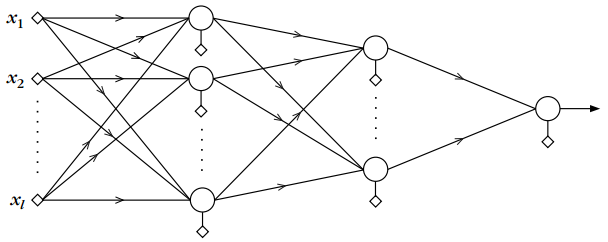
\includegraphics[width=\textwidth]{multilayer}
				\caption[Network with two hidden layers and single output neuron.]{Architecture of an artificial neural network with two hidden layers and a single output neuron \cite{theodoridis2008pattern}.}
				\label{fig:multilayer}
			\end{figure}		
		
			The way in which neural networks are usually programmed to perform a function is through a process of \emph{learning}, which typically involves modifying the synaptic weights in such a way as to attain the desired objective \cite{haykin2009neural}. As will be analysed in section~\ref{sec:constructive}, learning is not limited to that, as it is also possible for neural networks to modify their own topology, ability which is exploited by the current project.
		
			\newpage
		
			\begin{figure}[t]
				\centering
				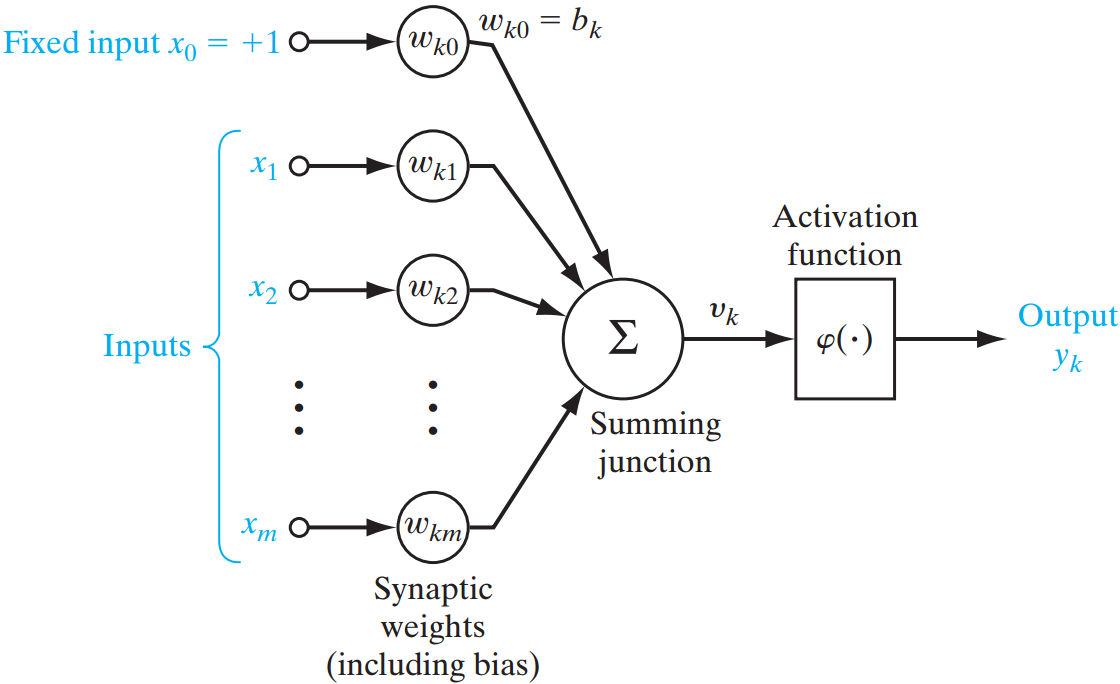
\includegraphics[width=0.85\textwidth]{neuron}
				\caption{Nonlinear model of a neuron \cite{haykin2009neural}.}
				\label{fig:neuron}
			\end{figure}
		
			Figure~\ref{fig:neuron} shows a representation of a generic model of an artificial neuron. In detail, its main components are:
			\begin{enumerate}
				\item A set of \emph{synapses} or \emph{connecting links}, characterized by a \emph{weight} or \emph{strength}. If a signal $x_j£$ is at the input of a synapse $j$ connected to a neuron $k$, the input signal gets multiplied by the synaptic weight $w_{kj}$.
				\item A \emph{sum} function $\Sigma$ which implements a \emph{linear combination} of the inputs with their respective synaptic weights.
				\item An \emph{activation} or \emph{transfer} function $\varphi$ which limits the amplitude of the output of the neuron, usually to the closed interval $[-1, 1]$. Nonlinear functions such as the \emph{sigmoid} are common choices.
				\item Optionally, the model can include a value $b_k$ called \emph{bias}, whose role is to increase or lower the net input of the activation function. This is usually implemented by having an additional, fixed input $x_0 = 1$ multiplied by its respective weight $w_{k0}$ \cite{haykin2009neural}.
			\end{enumerate}
		
			Mathematically, the behaviour of a neuron can be described by the following equations:
			\begin{equation}
				v_k = \sum_{j=0}^{m} w_{kj}x_j
			\end{equation}
			\begin{equation}
				y_k = \varphi(v_k)
			\end{equation}
		
			Nodes in a network are usually grouped into three classes: an \emph{input layer}, whose neurons receive the information to be processed; an \emph{output layer}, which yield the results of the processing; and neurons in between organized in zero or more \emph{hidden layers} \cite{kotsiantis2007supervised}.
		
			The representational power of neural networks is well defined theoretically: in fact, any continuous function can be implemented in a three-layer net, given sufficient number of hidden units, proper nonlinearities, and weights \cite{hornik1989multilayer,kuurkova1992kolmogorov,lam2015prslides}.
		
			\subsection{Network architectures}
				\subsubsection{Feedforward networks}
				The simplest type of topology is the feedforward network, which allows signals to travel only one way, from input to output \cite{kotsiantis2007supervised}; this layout is thus strictly acyclic. The signals resulting from the input layer are fed to the second layer, and so on till the final layer, whose output constitutes the overall response of the network to the source pattern \cite{haykin2009neural}.
				
				\begin{figure}[h]
					\centering
					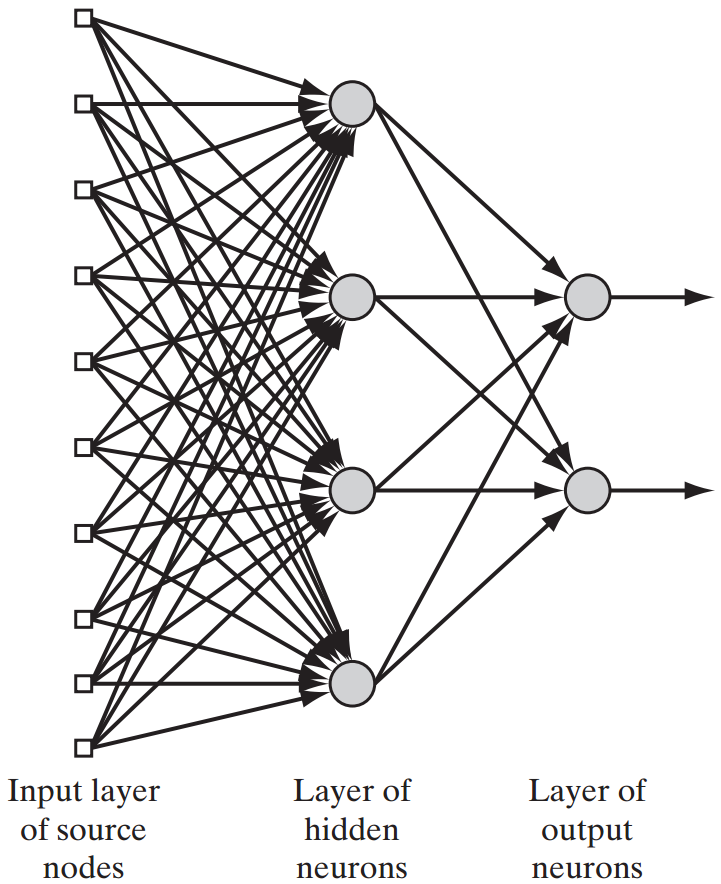
\includegraphics[width=0.6\textwidth]{feedforward}
					\caption{Fully connected feedforward neural network \cite{haykin2009neural}.}
					\label{fig:feedforward}
				\end{figure}
				
				Typically (but not necessarily) the neurons in each layer are only connected to the ones into the immediately following layer. If every node in each layer is connected to every other node in the adjacent layer, the neural network is said to be \emph{fully connected} (respectively \emph{partially connected}) \cite{haykin2009neural}. Figure~\ref{fig:feedforward} shows an example of such a network.
				
				\subsubsection{Recurrent networks}
				\nomenclature{RNN}{Recurrent Neural Network.}
				\begin{figure}[t]
					\centering
					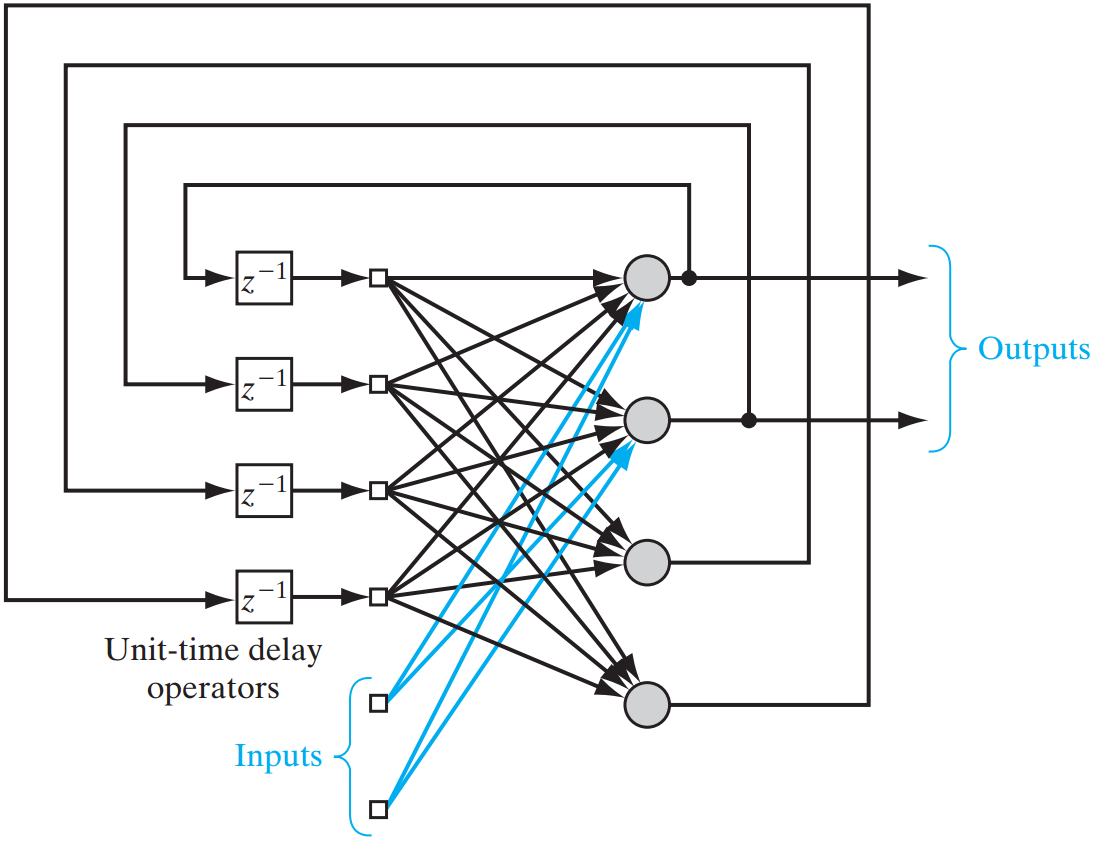
\includegraphics[width=0.9\textwidth]{recurrent}
					\caption{Recurrent neural network with hidden neurons \cite{haykin2009neural}.}
					\label{fig:recurrent}
				\end{figure}
				Contrarily to feedforward networks, \emph{recurrent} neural networks have at least one \emph{feedback} loop. Feedback is present in a system when the output of an element influences (at least in part), the input applied to that same element \cite{haykin2009neural}; connections among its neurons thus contribute to form a directed cycle in the topology \cite{yu2015recurrent}. The presence of these cycles has a deep impact on the learning capabilities of recurrent neural networks \cite{haykin2009neural}. The topology employed by the DIM algorithm makes use of feedback loops (see section~\ref{sec:negfeedback}).
				
				Recurrent networks are general computers, much more powerful than simple feedforward ones \cite{schmidhuber2015deep}; in fact, cycles account for the creation of an internal state which allows them to deal with temporal behaviour \cite{yu2015recurrent}. As a significant example, they have the ability to both create and recognize sequences of input patterns \cite{cleeremans1993mechanisms,pearlmutter1990dynamic}.
				
				\subsubsection{Deep networks}
				A \emph{deep} neural network is a neural network with multiple hidden layers. Even though, theoretically, \emph{shallow} (as opposed as deep) networks have the ability to represent every kind of function, in practice recent findings indicate that \emph{deep architectures} may be better suited to the task of representing some complicated functions (e.g. as those found in vision and language). Specifically, \emph{\quot{functions that can be compactly represented by a depth $k$ architecture might require an exponential number of computational elements to be represented by a depth $k - 1$ architecture}} \cite{bengio2009learning}.
			
				The main reason behind that and the motivation for deep networks is that those complex behaviours are modelled by mathematical functions which are highly nonlinear in terms of the input signals. The statistical relationships governing that extreme variability may be to complex and not readily deductible at that level. Therefore each hidden layer of the deep network is assigned with the task of extracting \emph{features} from the previous stage, in this way transforming the original input into increasingly more abstract representations \cite{bengio2009learning}.
				
				The PC/BC model on which the project is based (described in section~\ref{sec:pcbc}) in its general, hierarchical form can be considered a case of deep network.
		
			\subsection{Classes of training algorithms}
				The process of learning can be categorized in three distinct classes: \emph{supervised}, \emph{unsupervised}, and \emph{reinforcement learning}.
				
				In \emph{supervised learning}, training is performed on the basis of a set of input-output examples provided from an external source of knowledge. Input vectors are fed to the network and the resulting output is compared with the expected one; then, through a process called \emph{error-correction}, the weights of the network are modified in such a way as to minimize the error between the expected outcome and the actual output \cite{haykin2009neural}.
				
				In \emph{unsupervised learning}, no examples are provided and the training algorithm has to rely on a task-indipendent measure which quantifies the quality of the representation. The network is thus optimized with respect to that measure. Most unsupervised algorithms achieve training through \emph{competition} \cite{spratling2009unsupervised}: in this case, an input layer of neurons sends activations to a competitive layer, whose neurons compete for the chance to respond to features in the data. Therefore nodes which represent features in the data are made more likely to activate, according to a certain rule \cite{haykin2009neural}. Negative feedback networks (presented in section~\ref{sec:negfeedback}) employed by the DIM algorithm are an example of a model that provides competition.
				
				In \emph{reinforcement learning}, the network learns through interaction with the \emph{environment}: the result of the output is evaluated and the network is updated to minimize an \emph{index of performance}.	
		
		\newpage		
		
		\section{Negative Feedback Networks}
			\label{sec:negfeedback}
			\begin{figure}[h]
				\centering
				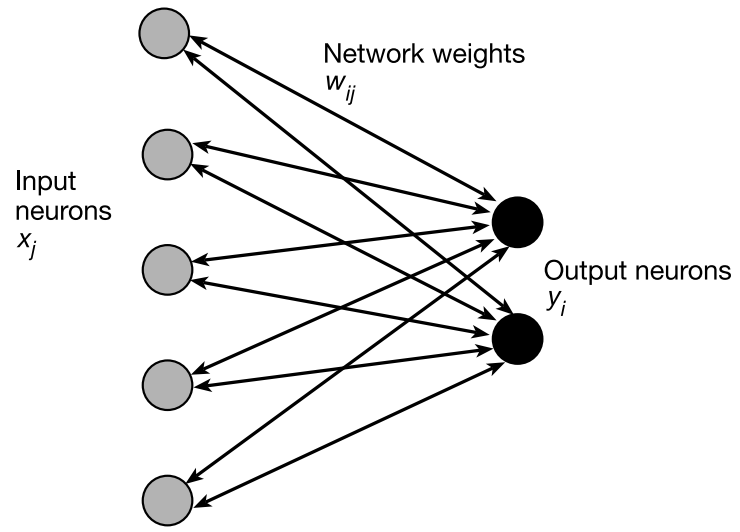
\includegraphics[width=0.7\textwidth]{negfeedback}
				\caption[Negative feedback network.]{Negative feedback network where the activation is fed forward from inputs $x$ through weights $W$ to outputs $y$. It is then fed back as subtractive \emph{inhibition} through the same weights \cite{charles1998modelling}.}
				\label{fig:negfeedback}
			\end{figure}
			Negative feedback networks are a model for unsupervised learning in which competition is achieved, rather than by lateral \emph{inhibition} (where nodes influence the output of other nodes), by inhibiting the inputs of the competing nodes. In this kind of networks, the activation of the output nodes is \emph{fed back} to their inputs and subtracted, effectively implementing the competition \cite{spratling2009unsupervised}, as in the example shown in figure~\ref{fig:negfeedback}.
		
			\subsection{Fyfe's Network}
				One good example of negative feedback network algorithm is the one described by Fyfe and his colleagues in \cite{charles1997discovering,charles1998modelling,charles2002unsupervised,fyfe1997neural}. These networks are based on the initial assumption that both weights and outputs can not be negative; constraints are thus set so that, if that happens, they are instead set to zero. The motivations behind this are that (1) the kind of data that is presented to the network will always be positive, so it is reasonable to expect the activity in the network to be positive as well, and (2) synapses in the brain are not believed to be able to change from excitatory to inhibitory \cite{charles1998modelling}.

				\newpage

				\begin{figure}[h]
					\centering
					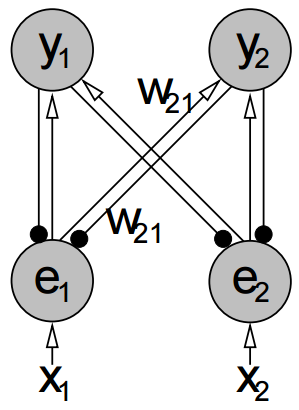
\includegraphics[width=0.3\textwidth]{basictopology}
					\caption[Basic model for the network studied in the project.]{Two-node, two-input neural network with inhibitory feedback. Excitatory synapses are shown as arrows while inhibitory ones as filled circles \cite{spratling2009unsupervised}. This is the basic form of all the model on which the algorithms involved in the project are based.}
					\label{fig:basictopology}
				\end{figure}

				If the network has $m$ inputs and $n$ competing nodes, then the equations regulating the activity of the networks are as following:
				\begin{equation}
					y = Wx
				\end{equation}
				\begin{equation}
					e = x - W^Ty
				\end{equation}
				\begin{equation}
					W \leftarrow W + \beta y e^T
				\end{equation}
				Where $y = [y_1, ..., y_n]^T$ represents the vector of the outputs,\\$x = [x_1, ..., x_m]^T$ the vector of inputs, $W = [w_1, ..., w_n]^T$ an $n$ by $m$ matrix of weights, with each row containing the weights received by a single node, and $e$ is the vector of inhibited inputs\footnote{As explained in the introduction (section~\ref{sec:background}), inhibited inputs can be equivalently interpreted as representing the \emph{reconstruction error} of the network, without any changes to the mathematical model \cite{spratling2009unsupervised}.}.
			
				The third equation describes the training rule, where $\beta$ is a parameter known as \emph{learning rate}. As it can be seen from all the equations, the inhibited inputs only influence the learning phase and not the output of the network directly, so this model does not fully implement competition which, in the application we are concerned of, results in the inability of the network to correctly represent the input, even when the weights have been correctly learned.
				
			\subsection{Harpur's Network}
				Harpur proposes a different algorithm based on the same model \cite{harpur1994fast,harpur1996development,harpur1997low} which does provide competition which influences the network output directly. The equations describing its behaviour are the following:
				\begin{equation}
					\label{eq:harpur_error}
					e = x - W^Ty
				\end{equation}
				\begin{equation}
					\label{eq:harpur_output}
					y \leftarrow y + \mu W e
				\end{equation}
				\begin{equation}
					W \leftarrow W + \beta y e^T
				\end{equation}
				As it can be seen, the learning rule is the same of the one used by Fyfe's algorithm. Note that weights are clipped to be in the range $[0,1]$. What is different from the previous case is how the values for $y$ and $e$ are calculated. First, and for each new input image, $y$ is initialized to zero; then equations \ref{eq:harpur_error} and \ref{eq:harpur_output} are iterated until they converge to the final value. Negative values of $y$ are clipped to zero at every iteration.
				
				The parameter $\mu$ has to be carefully chosen: big values will cause some elements of $y$ to grow too large in a single step, causing the values in $e$ responsible for the activation of those elements to decrease, and so on. Output values thus oscillate without reaching a steady-state. For this reason, $\mu$ has to be small, which however causes $y$ to be updated slowly, thus requiring many iterations to achieve convergence \cite{spratling2009unsupervised}.
	
		\section{Non-negative Matrix Factorisation}
			\nomenclature{NMF}{Non-negative Matrix Factorisation.}
			Non-negative matrix factorisation is a method to find two factors $W^T$ and $Y$ of a non-negative matrix $X$  \cite{spratling2009unsupervised}, such that:
			\begin{equation}
				X \approx W^T Y
			\end{equation}
			\begin{equation}
				\begin{split}
					W \nless 0 \\
					Y \nless 0
				\end{split}
			\end{equation}
			Since image components are non-negative, theoretically this is a suitable method to find parts-based decomposition of images \cite{feng2002local}. 
			
			If $m$ is the size of the images, $n$ is the number of possible image components, and $p$ is the number of images in the training set, then:
			\begin{itemize}
				\item $X = [x_1, ..., x_p]$ is an $m \times p$ matrix, with each column containing the pixels of a training image.
				\item $W^T$ is an $m \times n$ matrix of weight values, with each column being a component (or basis vector) into which an image can be decomposed.
				\item $Y = [y_1, ..., y_p]$ is an $n \times\ p$ matrix, with each column describing the activation of each component in the corrisponding training image.
			\end{itemize}
			An individual training image can be reconstructed as:
			\begin{equation}
				x_k \approx W^T y_k
			\end{equation}

			Non-negative matrix factorisation shares mathematical similarity with negative feedback neural networks. In particular, NMF can be seen as a \emph{divisory form} of feedback inhibition. However, the main difference is that NMF operates in batch mode, while negative feedback neural network is an on-line algorithm \cite{spratling2009unsupervised}. There exists a number of algorithms to approximate the solutions for that equation. Even so, all of them operate on all the training data at once.
			
			\subsection{Sequential version}
			In analogy to negative feedback networks, the term
			\begin{equation*}
				E = X \oslash (W^T Y)
			\end{equation*}
			which measures the residual error in the reconstruction of $X$, can be introduced. By performing the relevant substitutions and on the basis of some simplifying assumptions (detailed in \cite{spratling2009unsupervised}), the formulas can be rewritten and iterative rules for the vectors relative to a single training image (written in lowercase) can be derived:
			\begin{equation}
				\label{eq:nmf_error}
				e = x \oslash (\epsilon + W^T y)
			\end{equation}
			\begin{equation}
				y \leftarrow (\epsilon + y) \otimes (We) \oslash \tilde{w}
			\end{equation}
			\begin{equation}
				W \leftarrow W \otimes (1 + \beta y (e^T - 1))
			\end{equation}
			Where $\tilde{w}$ is a column vector each element of which represents the total synaptic weight received by one output node.
			
			Comparing equation~\ref{eq:nmf_error} with equation~\ref{eq:harpur_error}, the similarity between NMF and negative feedback networks is obvious: specifically, NMF implements a divisive, rather than subtractive, feedback.
			
			In contrast to Fyfe's networks, sequential NMF provides competition between the nodes of the network. Moreover, the resulting algorithm is more stable than Harpur's algorithm \cite{spratling2009unsupervised}.
	
		\newpage

		\section{PC/BC}
			\nomenclature{PC/BC}{Predictive Coding as Biased Competition.}
			\label{sec:pcbc}
			\subsection{Predictive coding}
				\begin{figure}[h]
					\centering
					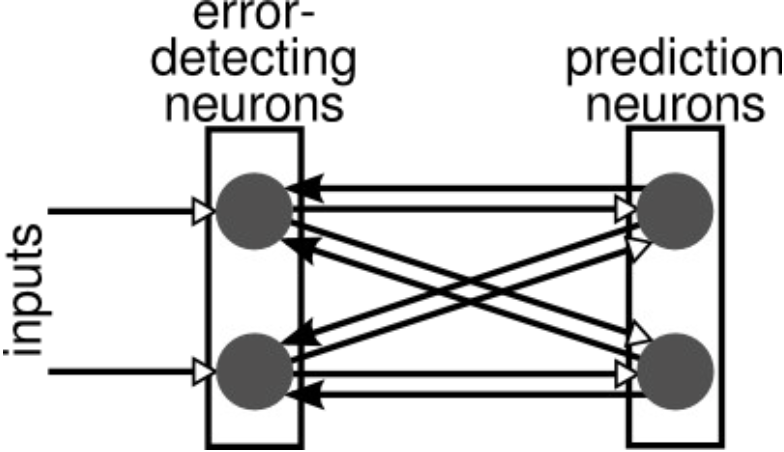
\includegraphics[scale=0.5]{prediction}
					\caption[Representation of pair of adjacent populations in PC model.]{A graphical representation of a pair of adjacent populations in the PC model. \cite{spratling2014predictive}.}
					\label{fig:predictive}
				\end{figure}
				
				Predictive coding is commonly used to model information processing in cerebral cortex. It is typically implemented as hierarchical neural networks with alternating populations of \emph{error-detecting} and \emph{prediction} neurons. Prediction neurons' activity produces a reconstruction of the inputs via feedback connections to the preceding error-detecting neurons; error-detecting neurons calculate the residual error between the reconstructed and the actual inputs \cite{spratling2014predictive}.
				
				By having the weights in a matrix $W$, its rows, each of which corresponds to the weights targeting a single prediction neuron, represent the \emph{elementary components} from which the images can be reconstructed. The strength of activation of the prediction neuron thus encodes the \emph{degree of belief} that that pattern of inputs is present in the current image \cite{spratling2014predictive}.
				
				The matrix $W$ can thus be thought as a \emph{dictionary}, a model of the external world \cite{spratling2012unsupervised,spratling2014predictive}.

				\begin{figure}[h]
					\centering
					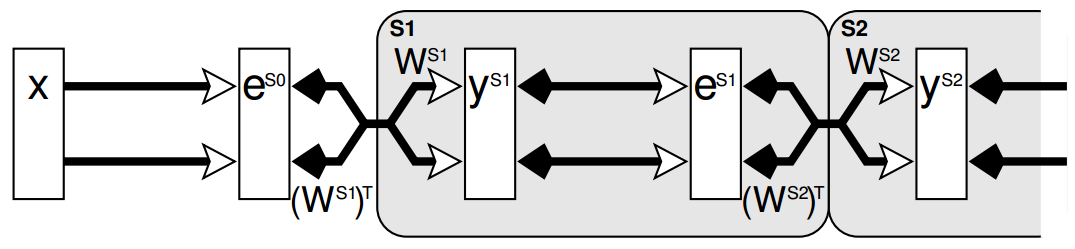
\includegraphics[width=\textwidth]{pc}
					\caption[Multi-stage, hierarchical predictive coding model.]{Multi-stage, hierarchical predictive coding model. Open arrows signify excitatory connections, filled arrows inhibitory ones \cite{spratling2008reconciling}.}
					\label{fig:pcbc}
				\end{figure}

			\subsection{Predictive coding as biased competition}
				\begin{figure}[h]
					\centering
					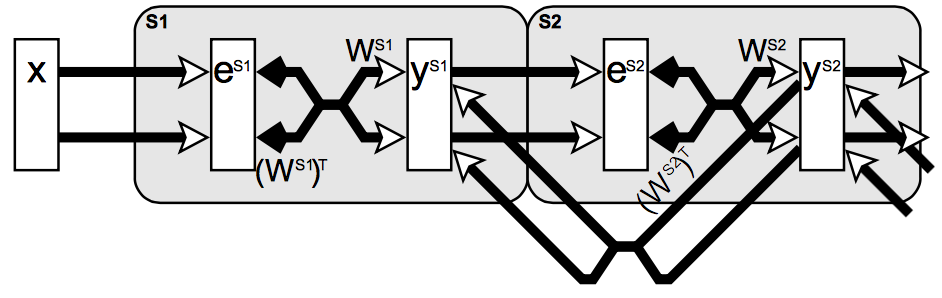
\includegraphics[width=\textwidth]{pcbc}
					\caption{A graphical representation of the PC/BC model \cite{spratling2008predictive}.}
					\label{fig:pcbc}
				\end{figure}
				
				\textcolor{red}{Expand.}
				
				PC/BC is an alternative model equivalent to PC but which uses direct excitatory feedback from one population of prediction nodes to the preceding one \cite{spratling2008predictive}.
				
				With some modifications, the rearranged model can be implemented by means of a negative feedback neural network as the ones analyzed previously \cite{spratling2008reconciling}.
				
		\section{Divisive Input Modulation}
			\label{sec:dim}
			\nomenclature{DIM}{Divisive Input Modulation.}
			Notwithstanding the improvements of the sequential NMF algorithm compared to Fyfe and Harpur's networks, the former still suffers from a weakness that makes it poor at learning image components when overlapping between components is present in the training images \cite{spratling2009unsupervised}.
			
			\begin{figure}[h]
				\centering
				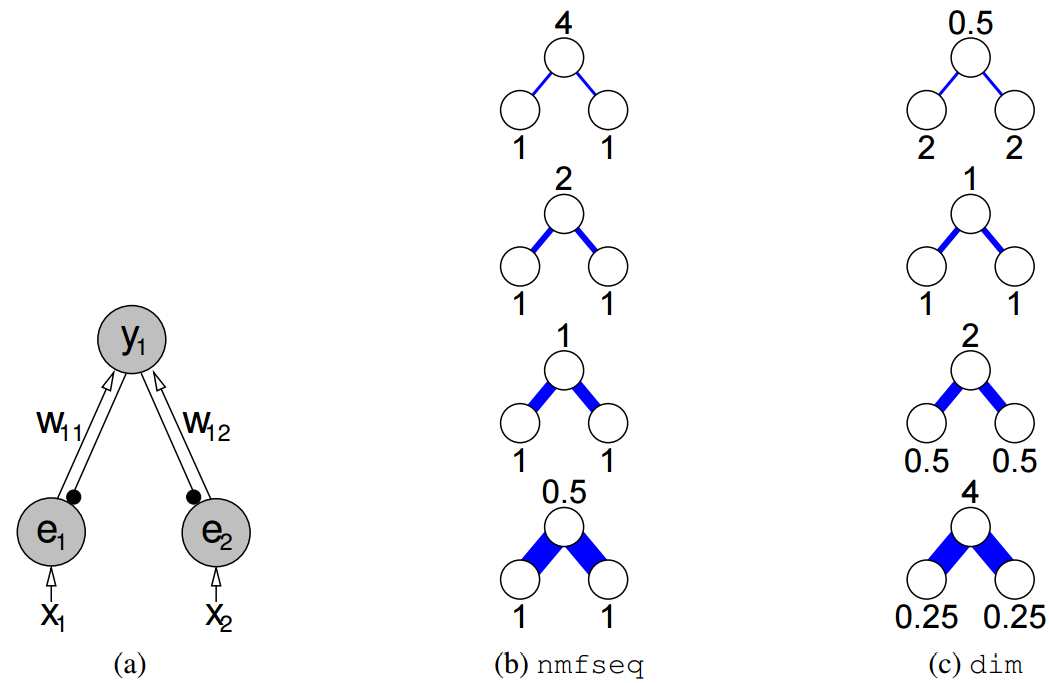
\includegraphics[width=0.85\textwidth]{nmf_problem}
				\caption[Graphical explanation of the NMF problem.]{\textcolor{red}{Describe the problem briefly. \cite{spratling2009unsupervised}}}
				\label{fig:nmf_problem}
			\end{figure}	
					
			The problem is illustrated by figure~\ref{fig:nmf_problem}. Intuitively, one might expect that as the strengths of the weights increase, so would the response of the output node. In sequential NMF however, as the weights increase the output node inhibits the input it receives more strongly, and the response actually decreases. To fix this behaviour, Spratling \cite{spratling2009unsupervised} proposes an algorithm called \emph{Divisive Input Modulation}, which is the one on which the current project is based on. The algorithm makes use of the following equations:
			\begin{equation}
				e = x \oslash (\epsilon + \hat{W}^T y)
			\end{equation}
			\begin{equation}
				y \leftarrow (\epsilon + y) \otimes We
			\end{equation}
			\begin{equation}
				W \leftarrow W \otimes (1 + \beta y (e^T - 1))
			\end{equation}
			Where $\hat{W}$ is a matrix representing the same synaptic weight values as $W$ but with rows normalised to have a maximum value of 1, and $\epsilon$ is a small constant used to prevent division-by-zero errors. Following learning, weights are clipped at zero.
			
			\textcolor{red}{Expand on why the problem is fixed.}
			
			Divisive Input Modulation showed results superior to existing methods in learning image components, especially in the presence of occlusion and overlapping \cite{spratling2009unsupervised}.
			
			\subsection{PC/BC--DIM}
				\textcolor{red}{Expand.}
				
				Activation rules for a PC/BC model as the one in figure~\ref{fig:pcbc} implemented as a hierarchical neural network are as follows:
				
				$$e^{Si} = G(y^{Si-1}) \oslash [\epsilon_2 + (V^{Si})^T y^{Si}]$$
				$$y^{Si} \leftarrow (\epsilon_1 + y^{Si}) \otimes W^{Si}e^{Si} \otimes [1 + \eta G((U^{Si+1}))^T y^{Si+1}]$$
				
				Where:
				\begin{itemize}
					\item $Si$ indicates the stage $i$ of the hierarchical network.
					\item $e^{Si}$ is a $m \times 1$ vector of error-detecting neuron activations.
					\item $y^{Si}$ is a $n \times 1$ vector of prediction neuron activations.
					\item $W^{Si}$, $V^{Si}$, $U^{Si}$ are $n \times m$ matrces of synaptic weights.
					\item $\epsilon_1$, $\epsilon_2$, $\eta$ are parameters.
					\item $G$ is a function that clips values at 1. 
				\end{itemize}
				
				In the first equation, the first term represent the actual input, while the second term represents the reconstructed input from the prediction neurons.
				
				In the second equation, the first term represents the previous value of $y^{Si}$, the second term is the feedforward input from error-detecting neurons to prediction ones, and the third term represents the modulation coming from the top-down predicitions of the next stage, if any.
				
		\section{Constructive Neural Networks}
		\label{sec:constructive}
			\emph{Constructive algorithms} are used to adjust the structure of a neural network during the learning phase. Different approaches are possible: a purely constructive one adds layers, neurons and connections starting from a minimal architecture, whereas \emph{pruning} starts from a complex structure and removes redundant parts; the two approaches can also be combined \cite{parekh2000constructive}.
					
			The advantages of using a constructive algorithm are, among the others:
			\begin{itemize}
				\item It is flexible: the whole space of possible neural network configurations can be explored.
				\item The initial configuration of the model is minimal and straightforward.
				\item Final configurations can be thought as estimating the real complexity of the learned problem.
			\end{itemize}
					
			The two main branches of constructive algorithms are Cascade Correlation (CC) and Dynamic Node Creation (DNC):
			
			The CC algorithm produces neural networks with multiple hidden layers, with one neuron each that is connected to all other neurons previously added \cite{sharma2010constructive}.
					
			DNC add neurons in a hidden layer until the network achieves an approximation of the desired performances.
			Every time a neuron is added, all the weights are retrained. This is effective but at the expense of computational cost. \cite{sharma2010constructive}
					
			OHL-FNN is an extension of DNC that freezes the neural network weights that have been previously trained, and that retrains only the weights affected by the insertion \cite{kwok1997objective}.

	
	\chapter{Main Result}
		\section{Analysis and Design}
			\subsection{Motivation}
				There are various advantages in developing a constructive neural network algorithm over a standard one; some of them are obvious while some of them are more subtle.
				
				First of all, as stated in the introductory section, differences in architecture and size can be all the difference needed in making a network useful for the problem. In this field, choices are often the result of trial and error and, as such, often result in designs which are larger than what would be actually needed \cite{?}. This has two main repercussions on the performance of the network.
				
				On one hand, training a bigger network is computationally more expensive. On the other hand, models with too many degrees of freedom, while they can perform more complicated mappings, tend to overfit the training data and are not able to perform well over unseen instances. This ability, called \emph{generalization}, implies lower order mappings \cite{alpaydin1994gal}.
				
				An analogy with the problem of curve fitting using polynomials serves to illustrate the point: a polynomial with too few coefficients will be unable to capture the underlying function, while a polynomial with too many coefficients will fit the noise in the data and also result in a poor representation of the function. On the contrary, the optimal number of coefficients will result in the best representation of the function and also the best predictions for new data \cite{kwok1997objective}. Constructive algorithms solve this problem by incorporating the evolution of the network structure into the learning algorithm.
				
				Less obviously, but importantly, algorithms that prefer small solutions have the possibility to discover a minimal (or near-minimal) network which potentially suits the intrinsic complexity of the learning task \cite{parekh2000constructive}.

			\subsection{Analysis of the current algorithm}
				The details of the Divisive Input Modulation algorithm and the theory on which is based have already been discussed in section~\ref{sec:dim}; in this subsection we are only interested in focusing on the aspects that are most relevant in the design of its constructive version.

				\begin{figure}[h]
					\centering
					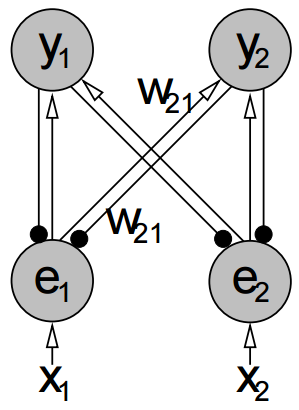
\includegraphics[width=0.3\textwidth]{basictopology}
					\caption{Basic structure of the neural network used by DIM \cite{spratling2009unsupervised}.}
					\label{fig:dim}
				\end{figure}

				Specifically, we should analyse the parameters involved, to discover which ones makes sense to modify at runtime and which ones offer information useful for the constructive process. The $m$ pixels in the images, indicated by $x_1, ..., x_m$, which are mapped one-to-one to the \emph{error-detecting} neurons ($e_1, ..., e_m$) are fixed parameters depending on the training set. The part of the network that can be grown or shrunk in size is the output or \emph{predictive} layer ($y_1, ..., y_n$) and, consequently, the number of rows in the matrix of weights $W$; in short, the parameter $n$.
				
				A question which is important to answer is: what does tuning this parameter means in terms of image decomposition? As it is known from the literature \cite{spratling2014predictive}, the weights received by a single output neuron are contained in the respective row in the matrix $W$; each row corresponds to an elementary component discovered in the image. So tuning the parameter $n$ equals to identify the exact number of components needed to describe the images in the training set.
				
				Another important point is: what factor should drive the decision of adding neurons to the network? The way the algorithm is engineered, the values of the error-detecting neurons provide an estimation of how accurately the generative model is reconstructing the original input, and thus explaining its composition. Specifically, when a value within $e$ is greater than 1, the corresponding element in the input is under-represented in the reconstruction, whereas if that value is less than 1, the opposite true. The interpretation of the image is perfect if $e$ is equal to 1. So it makes perfect sense to somehow consider by how far the values of $e$ are from the unity in order to approximate the accuracy the network has reached.
			
				\textcolor{red}{Talk about the fact that the network is fully connected.}
				
			\subsection{Classes of constructive algorithms}
				\nomenclature{CC}{Cascade Correlation.}
				\nomenclature{DNC}{Dynamic Node Creation.}
				
				\textcolor{red}{Pruning and why purely constructive is better.}
				
				According to \cite{fernandes2014constructive}, two main approaches can be identified in the development of constructive neural network algorithms: they are \emph{Cascade Correlation} (CC) and \emph{Dynamic Node Creation} (DNC). Cascade Correlation and its derived algorithms are not suited for the problem at hand, as they create neural networks with multiple hidden layers, whereas DIM expects a single constructive layer to grow in the number of neurons.
				
				For this reason, the class of algorithms known as DNC was considerate more appropriate for the task. The original model proposed by Ash \cite{ash1989dynamic} is quite simple: the algorithm adds neurons to the designated layer until the precision of the output reaches the desired level. The entire neural network is retrained every time a neuron is added.
				
				Even though these algorithm were conceived for simple feed forward neural networks, they have been proven successful even when applied to recurrent networks \cite{ash1989dynamic}.
				
			\subsection{Criteria for adding neurons}
				One of the main decisions to be made when designing a constructive algorithm is under what conditions should new neurons be added to the network.
				
				At first, I experimented with a very simple criterion: simply add a neuron if the overall average error, measured as the absolute distance from 1 among all the elements of $e$ and for one epoch, is higher than a certain threshold. Results were not very good and the network tended to grow bigger and bigger, which initially led me to introduce a pruning phase to overcome the problem. As stated in section \textcolor{red}{section}, pruning is an inherently inferior solution compared to constructive, so I moved forward to explore different approaches.
				
				An analysis of the shape of a typical curve describing the overall squared error in the network over time will help in deriving a better criterion. First of all, note that the error monotonically decreases over time. However, at some point the learning tends to reach a plateau and any further improvement will follow the rule of diminishing returns \cite{ash1989dynamic}. Just before that happens is the right moment when to change the topology of the network (i.e. adding a neuron) to prevent the plateau to occur.
				
				Mathematically, if:
				\begin{itemize}
					\item $a_t$ is the average squared error at time \emph{t} across all the network,
					\item $t_0$ is the time when the last node was added,
					\item $t$ is the current time,
					\item $w$ is the size of the time window over which the slope is evaluated,
					\item $\Delta_T$ is the \emph{trigger slope}, namely the value of the slope under which a neuron is added,
				\end{itemize}
				then a neuron is added to the network if the following conditions are met:
				\begin{equation}
					\label{eq:slope}
					\frac{\left| a_t - a_{t-w} \right|}{a_{t_0}} < \Delta_T
				\end{equation}
				\begin{equation}
					\label{eq:topology}
					t - w \geq t_0
				\end{equation}
				Equation~\ref{eq:slope} detects when the error curve gets into a plateau, according to the user-set parameter $\Delta_T$, while equation~\ref{eq:topology} ensures that the first one always deals with the same topology.
				
				\begin{figure}[h]
					\centering
					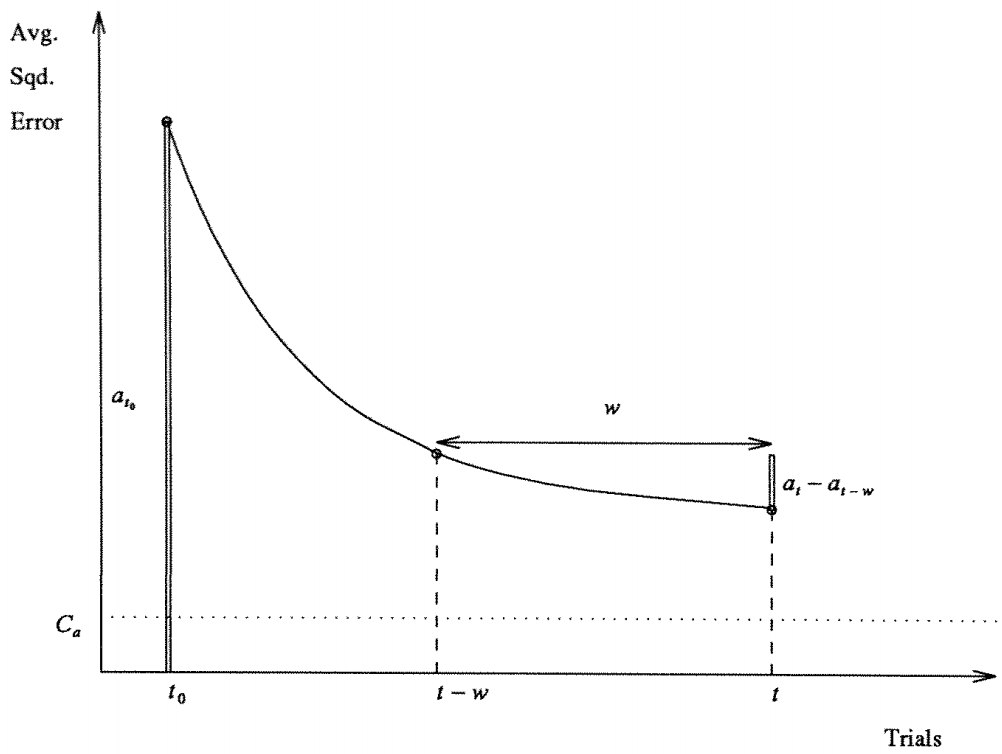
\includegraphics[width=0.9\textwidth]{error}
					\caption{Graphic of the overall error as a function of training time \cite{ash1989dynamic}.}
					\label{fig:error}
				\end{figure}
				
				This proved to be a much better measure than the original one, however the network would still keep growing indefinitely, trying to get a lower error even when the mapping is learned. Clearly, criteria for when to stop adding neurons to the network are needed. So, the algorithm will not add any nodes no matter what once the average error goes under a certain specified threshold:
				
				\begin{equation}
					a_t \leq C
				\end{equation}
				
				where $C$ is the over-mentioned, user-defined threshold.
				
				With the last modification, the algorithm performed fairly well, however there was still room for improvement. Specifically, as it is not possible to know \emph{a priori} how big the network is going to be, the algorithm has to start with the smallest possible network, which is the one with a single predictive neuron. However, it can take various iterations to bring the network to an adequate size, especially if the number of components which make up the images is high.
				
				Intuition suggests, and experiments have confirmed, that when the number of neurons in the network is largely inadequate to describe the images, then error-detecting neurons are going to yield values whose distance from the unity (and thus from correct representation) is very high. In this case, and thus if the error is over a certain threshold, the algorithm increases the number of neurons by a multiplicative factor until it goes under that threshold. It then starts behaving as described early, i.e. by adding neurons one at a time. This procedure is inspired by the TCP congestion control algorithm \cite{allman2009tcp}, in particular by its \emph{{exponential growth}} phase.
				
			\subsection{Division in epochs}
				To efficiently implement the concept of the \emph{window}, explained in the previous section, I decided to modify the original algorithm, by dividing the training procedure in \emph{epochs}. Throughout an epoch, each of which is constituted by a tunable number of cycles, the average of the error across the training set is kept updated. At the end of an epoch, and before starting the next one, the previously mentioned criteria are checked and the topology of the network modified accordingly, if necessary.
			
			\subsection{Weight training}
				Another outstanding question is how should weight training occur when the network grows in size? From the point of view of computational efficiency, and assuming that the units already present in the network are useful in part of the reconstruction \cite{kwok1997objective}, it would make sense to implement \emph{weight freezing}, that is, keeping the weights targeting the already existing neurons fixed, and allowing the new ones to vary.
				
				However, a case is made by Ash \cite{ash1989dynamic} that holding the existing network values constant only allows finding a solution in an affine subset of the weight space. The experiments I performed confirmed this thesis and the final version of my algorithm thus retrains whole the weights after each topology update.
			
		\section{Implementation}
			
		\section{Results}
			In order to assess the quality of the results, the algorithm has been tested against two sets of benchmarks: the \emph{squares} problem and the \emph{bars} problem.
			
			Both problems test the ability of the algorithm to learn the component parts from which a set of artificial training images are composed \cite{spratling2009unsupervised,spratling2012unsupervised}. The tests focus on three aspects: accuracy of the recognition, size of the network and training time.
			
			\subsection{Divisive Input Modulation}
				\subsubsection{Squares problem}
				\begin{figure}[h]
					\centering
					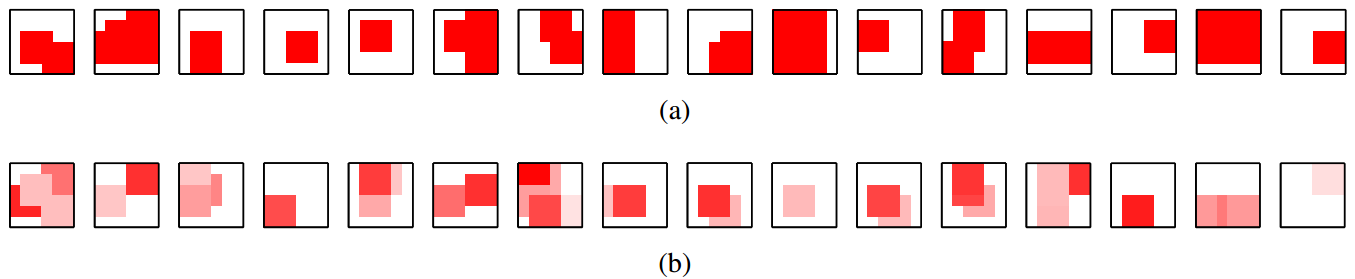
\includegraphics[width=0.9\textwidth]{squares}
					\caption{Example of 6-by-6 pixel images generated from 3-by-3 pixel square components \cite{spratling2009unsupervised}.}
					\label{fig:error}
				\end{figure}
				The squares problem is a more challenging variation of the bars problem with more significant overlapping between components. Each image in the dataset is generated by selecting, at random, elements from a fixed set of elementary image components, which are all $s$-by$s$ pixel squares. Each component gets assigned a probability regulating the frequency of appearance in the dataset; for each image, every selected component gets randomly assigned a \emph{contrast} and a (unique) \emph{depth}. Each pixel in the image thus gets a greyscale value corresponding to the contrast of the foremost square in that location, if any.
				
				The algorithms try to identify the components from which the dataset has been composed.
				
				\subsubsection{Results}
				\begin{table}[h]
					\centering
					\begin{tabular}{l*{4}{c}}
						Algorithm         & Accuracy & Cycles & Training time & Neurons \\
						\hline
						DIM               & 100\%    & 20000  & 18.9770s      & 48      \\
						Constructive DIM  & 100\%    & 20000  & 42s           & 48      \\
					\end{tabular}
					\caption{Performances as measured in a dataset of 6-by-6 pixel images with 3-by-3 pixel components.}
					\label{tab:performance}
				\end{table}
				
			\subsection{PC/BC--DIM}
				\subsubsection{Bars problem}
				\subsubsection{Results}
		
		\section{Discussion}
		
	\chapter{Conclusions}
	
	\bibliographystyle{plain}
	\bibliography{references}
	\nocite{*}
	
	\begin{appendices}
		\chapter{Source Code}
	\end{appendices}
\end{document}
